\documentclass[11pt,a4paper]{article}
\usepackage[T1]{fontenc}
\usepackage[utf8]{inputenc}
\usepackage{lmodern,microtype}
\usepackage[margin=27mm]{geometry}
\usepackage{amsmath,amssymb,amsthm}
\usepackage{enumitem}
\usepackage{booktabs}
\usepackage{tikz}
\usepackage[colorlinks=true,linkcolor=blue!45!black,urlcolor=blue!45!black,citecolor=blue!45!black]{hyperref}
\hypersetup{pdftitle={Which pictures can a woven heart show?},
  pdfauthor={Thomas Dybdahl Ahle}}
\newtheorem{theorem}{Theorem}
\newtheorem{lemma}[theorem]{Lemma}
\newtheorem{proposition}[theorem]{Proposition}
\newtheorem{corollary}[theorem]{Corollary}
\theoremstyle{definition}
\newtheorem{definition}[theorem]{Definition}
\theoremstyle{remark}
\newtheorem{remark}[theorem]{Remark}
\newcommand{\A}{\mathcal{A}}
\newcommand{\B}{\mathcal{B}}
\newcommand{\intr}{\operatorname{int}}
\newcommand{\bd}{\partial}
\definecolor{paper}{HTML}{B72B3C}
\definecolor{cutA}{HTML}{007CA8}
\definecolor{cutB}{HTML}{DF791B}
\definecolor{hid}{HTML}{3A7D44}
\setlist{itemsep=2pt,topsep=4pt,leftmargin=*}
\setlength{\emergencystretch}{1.5em}
\title{Which pictures can a woven heart show?}
\author{Thomas Dybdahl Ahle}
\date{November 2026}

\begin{document}
\maketitle
\begin{abstract}
A woven paper heart is made of two slitted sheets whose strips pass over and
under each other. Seen from the front it shows a picture in two colours.
We ask which pictures can arise. In the usual model, where the cuts of the
two sheets may cross, touch and run together, the answer is a local
condition: wherever the picture's boundary meets itself, exactly four pieces
meet, and it reaches opposite sides of the square equally often (and, with
one degenerate exception, that is all). So every reasonable picture can be
woven, and this is decided in linear time. The
proof is elementary: one sheet is cut almost arbitrarily, and the other is
repaired with two local moves. The stretches where the two cuts run together
are invisible in the finished heart, and they are what a designer pays
with. We show that $\Omega(n^2)$ of them are sometimes needed, that deciding
whether a picture needs none at all is NP-complete, and we list the
smallest pictures by the number they need.
\end{abstract}

\section{Hearts, cuts and pictures}

A woven heart (Danish \emph{flettet julehjerte}) is made from two pieces of
glossy paper of different colours. Each is folded and cut into strips from
the fold; the strips of one are then woven through the strips of the other.
The woven part is a square, and it is all we look at. Classic hearts have
straight cuts and show a checkerboard. Curved cuts give stars, animals and
letters, and the question of which pictures can be made at all is an old one
among the people who design them. Mogensen \cite{mogensen} describes the
model we use, and observes the device that makes most pictures possible:
where a cut of one sheet lies exactly on a cut of the other, the weave shows
nothing.

\paragraph{The model.}
Let $Q$ be a closed square with sides $T$, $R$, $B$, $L$ (top, right,
bottom, left). Everything is piecewise linear. The first sheet is cut along
a family $\A$ of $k$ pairwise disjoint simple arcs, each from the interior
of $T$ to the interior of $B$; the second along a family $\B$ of $l$
pairwise disjoint simple arcs, each from the interior of $L$ to the
interior of $R$. Every arc is \emph{proper}: it meets $\bd Q$ in its two
endpoints only. An arc of $\A$ and an arc of $\B$ may cross, touch, or
share subarcs.

The arcs of $\A$ cut $Q$ into $k+1$ strips, numbered $0,\dots,k$ from the
left; let $a(p)$ be the number of the strip of a point $p$ off $\A$, and
define $b(p)\in\{0,\dots,l\}$ likewise for $\B$, counting from the top.
Strips alternate over and under, so the colour seen at $p$ is
\[
  c(p) \;=\; a(p)+b(p)+\varphi \pmod 2 ,
\]
where the \emph{phase} $\varphi\in\{0,1\}$ says which sheet is on top in the
top left corner. We call $(\A,\B,\varphi)$ a \emph{weave} and the closure of
$\{c=1\}$ its \emph{picture}.

\begin{figure}[ht]
\centering
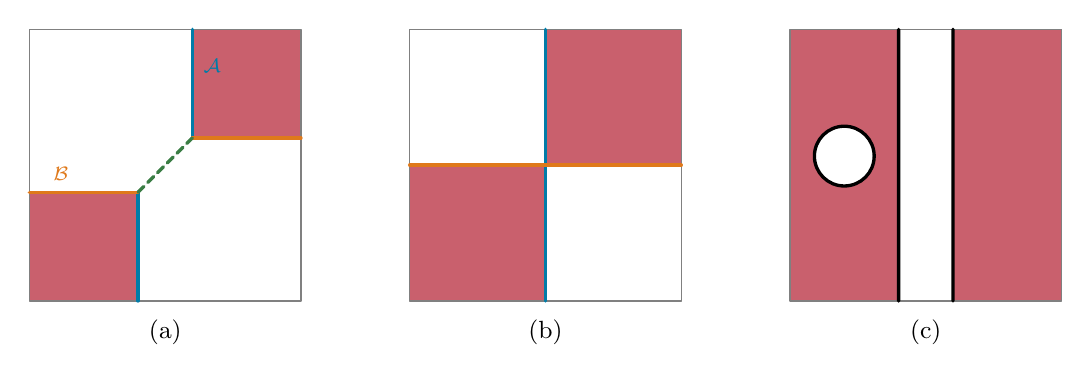
\begin{tikzpicture}[scale=1.15,line cap=round,line join=round]
\begin{scope}
\fill[paper!75] (1.8,3)--(3,3)--(3,1.8)--(1.8,1.8)--cycle;
\fill[paper!75] (0,0)--(1.2,0)--(1.2,1.2)--(0,1.2)--cycle;
\draw[gray] (0,0) rectangle (3,3);
\draw[cutA,very thick] (1.8,3)--(1.8,1.8) (1.2,1.2)--(1.2,0);
\draw[cutB,very thick] (0,1.2)--(1.2,1.2) (1.8,1.8)--(3,1.8);
\draw[hid,very thick,densely dashed] (1.2,1.2)--(1.8,1.8);
\node[font=\small] at (1.5,-.35) {(a)};
\node[font=\scriptsize,cutA] at (2.02,2.6) {$\A$};
\node[font=\scriptsize,cutB] at (.35,1.4) {$\B$};
\end{scope}
\begin{scope}[xshift=4.2cm]
\fill[paper!75] (1.5,3)--(3,3)--(3,1.5)--(1.5,1.5)--cycle;
\fill[paper!75] (0,0)--(1.5,0)--(1.5,1.5)--(0,1.5)--cycle;
\draw[gray] (0,0) rectangle (3,3);
\draw[cutA,very thick] (1.5,3)--(1.5,0);
\draw[cutB,very thick] (0,1.5)--(3,1.5);
\node[font=\small] at (1.5,-.35) {(b)};
\end{scope}
\begin{scope}[xshift=8.4cm]
\fill[paper!75] (0,0) rectangle (3,3);
\fill[white] (1.2,0) rectangle (1.8,3);
\fill[paper!75] (.35,1.9) circle (.0);
\fill[white] (.6,1.6) circle (.33);
\draw[gray] (0,0) rectangle (3,3);
\draw[black,very thick] (1.2,0)--(1.2,3) (1.8,0)--(1.8,3) (.6,1.6) circle (.33);
\node[font=\small] at (1.5,-.35) {(c)};
\end{scope}
\end{tikzpicture}
\caption{(a) A weave with one cut in each sheet. The cuts run together
along the dashed stretch, which the picture does not show: the white band
passes through it. (b) The same cuts crossing give a checkerboard. (c) A
picture no heart can show: its boundary never reaches the left or right
side, so the second sheet has no cuts, and the first cannot draw a circle.}
\label{fig:model}
\end{figure}

\paragraph{What the picture shows.}
Crossing an arc of $\A$ changes $a$ by one, and crossing an arc of $\B$
changes $b$ by one. So the colour changes exactly across the points that lie
on an arc of one family but not of the other. Write $\A$ and $\B$ also for
the unions of the arcs, and let
\[
  \Gamma \;=\; \overline{\A\,\triangle\,\B}
\]
be the closure of their symmetric difference: the \emph{visible} cuts. A
component of $\A\cap\B$ that is an arc is a \emph{hidden cut}; the colour is
the same on both sides of it (Figure~\ref{fig:model}a). The endpoints of a
hidden cut are its \emph{switches}.

\begin{definition}
A \emph{picture} is a closed set $M\subseteq Q$, a finite union of polygons,
that is the closure of its interior. Its \emph{boundary} $\Gamma(M)$ is the
closure of the frontier of $M$ inside $\intr Q$; it is a finite plane graph
whose vertices are the points of $\Gamma\cap\bd Q$ and the points where
$\Gamma$ is not locally an arc. A point of $\intr Q$ where four pieces of
$\Gamma$ meet is a \emph{touching}: two black regions meet there corner to
corner. An \emph{edge} of $\Gamma$ is a maximal arc between vertices, or a
closed curve of $\Gamma$ without vertices. $M$ is \emph{weavable} if it is
the picture of some weave. For a side $X$ we write $t_X=|\Gamma\cap X|$.
\end{definition}

A picture and its complement have the same boundary, and a weave for one
becomes a weave for the other by changing the phase. So weavability is a
property of $\Gamma$, and we mostly work with $\Gamma$.

\section{The criterion}

\begin{theorem}\label{thm:main}
A picture $M$ with boundary $\Gamma$ is weavable if and only if
\begin{enumerate}[label=\textup{(\roman*)}]
\item $\Gamma$ contains no corner of $Q$, and each point of
  $\Gamma\cap\bd Q$ is the end of exactly one edge;
\item every other vertex of $\Gamma$ is a touching;
\item $t_T=t_B$ and $t_L=t_R$; call these numbers $k$ and $l$;
\item if $l=0$ then $\Gamma$ consists of $k$ disjoint arcs from $T$ to $B$,
  and if $k=0$ of $l$ disjoint arcs from $L$ to $R$.
\end{enumerate}
\end{theorem}

Conditions (i) and (ii) are local, and (iii) is a count. When the boundary
reaches all four sides, (iv) is void: then \emph{any} picture, with islands,
rings inside rings, and regions of any shape, can be woven. Condition (iv)
is the one exception (Figure~\ref{fig:model}c). All four conditions are
checked in one pass over $\Gamma$, so weavability is decided in time linear
in the size of $\Gamma$.

A picture that fails (ii) has a point where three or more black regions
meet. Moving them apart slightly repairs it. A picture that fails (iii) can
be repaired by letting one more piece of its boundary run out to a side.
In this sense the theorem says that every picture is weavable after a small
change, which is what designers have found in practice.

\begin{proof}[Proof of necessity]
Let $M$ be the picture of a weave. Only arcs of $\A$ reach $T$ and $B$; they
are disjoint and proper, and arcs of $\B$ stay away from $T\cup B$. So near
a point of $T$ or $B$ the visible cuts are one arc end or nothing, and that
arc end is an end of an arc of $\A$. The same holds on $L$ and $R$ with
$\B$. This gives (i), and it shows that $\Gamma\cap T$ and $\Gamma\cap B$
are the two sets of endpoints of $\A$, so $t_T=t_B=k$; likewise
$t_L=t_R=l$. For (ii), at most one arc of each family passes through a
point, and each contributes at most two visible pieces there, so at most
four pieces of $\Gamma$ meet; the colour alternates around the point, so
their number is even. For (iv), if $l=0$ there is no $\B$, so nothing is
hidden and $\Gamma=\A$.
\end{proof}

When $l=0$ and (iv) holds, $\Gamma$ itself is the family $\A$, and likewise
when $k=0$. The rest of this section proves sufficiency for $k,l\ge 1$.

\subsection{Configurations and two moves}

Fix a picture satisfying (i)--(iii) with $k,l\ge1$. Number the points of
$\Gamma\cap T$ as $T_1,\dots,T_k$ from the left and those of $\Gamma\cap B$
as $B_1,\dots,B_k$ from the left; number $L_1,\dots,L_l$ and
$R_1,\dots,R_l$ from the top.

The idea is to give up, for a while, the demand that the second sheet's cuts
are $l$ arcs from $L$ to $R$. We ask only that they form disjoint curves.

\begin{definition}\label{def:config}
A \emph{configuration} is a pair $(\A,\B)$ of subsets of $Q$ such that
\begin{enumerate}[label=\textup{(C\arabic*)}]
\item $\A$ is a union of $k$ disjoint simple proper arcs, the $i$th from
  $T_i$ to $B_i$;
\item $\B$ is a compact $1$-manifold: a disjoint union of simple closed
  curves in $\intr Q$ and simple proper arcs, whose endpoints are exactly
  the points $L_1,\dots,L_l,R_1,\dots,R_l$;
\item $\overline{\A\triangle\B}=\Gamma$, and $\A\cap\B$ consists of the
  touchings and of finitely many disjoint arcs, the hidden cuts, whose
  interiors miss $\Gamma$ and whose ends are interior points of edges of
  $\Gamma$;
\item every edge of $\Gamma$ contains a subarc that lies in $\A$.
\end{enumerate}
\end{definition}

In a configuration every point of $\Gamma$, apart from switches and
touchings, lies in exactly one of $\A$ and $\B$. We call a subarc of an edge
of $\Gamma$ \emph{$a$-visible} if it lies in $\A$ and \emph{$b$-visible} if
it lies in $\B$. So $G=\Gamma\cup\A\cup\bd Q$ is a plane graph whose edges
in $\intr Q$ are of three kinds: $a$-visible, $b$-visible and hidden. Its
\emph{faces} are the components of $Q\setminus G$.

\begin{lemma}\label{lem:done}
If $(\A,\B)$ is a configuration in which $\B$ consists of $l$ arcs, the
$j$th from $L_j$ to $R_j$, then $M$ is weavable.
\end{lemma}
\begin{proof}
$\A$ and $\B$ are families as in the model, so with either phase they form
a weave. Its colour changes exactly across
$\overline{\A\triangle\B}=\Gamma$, so its picture is $M$ or the closure of
the complement of $M$; choose the phase accordingly.
\end{proof}

Three local facts about a configuration will be used repeatedly.

\begin{lemma}\label{lem:local}
\begin{enumerate}[label=\textup{(\alph*)}]
\item At a switch $p$, the edge of $\Gamma$ through $p$ is $a$-visible on
  one side of $p$ and $b$-visible on the other.
\item Every hidden cut is an arc of a component of $\B$, and at each of its
  ends that component continues along the $b$-visible side.
\item The boundary of every face of $G$ contains an $a$-visible or a hidden
  piece.
\end{enumerate}
\end{lemma}
\begin{proof}
(a) Three edges of $G$ meet at $p$: the hidden cut $h$ and the two parts
$f^-$, $f^+$ of the edge of $\Gamma$. The point $p$ is interior to an arc of
$\A$, which contains $h$, so exactly one of $f^\pm$ lies in $\A$. The same
holds for $\B$, and each of $f^\pm$ lies in exactly one of the two.
(b) follows, since no arc of $\A$ is closed and so no hidden cut is.
(c) Let $U$ be a face with no such piece on its boundary. Since $k\ge 1$,
$U\neq\intr Q$, so $\bd U$ contains a point $z$ in the interior of an edge
$f$ of $\Gamma$, and $f$ is $b$-visible at $z$. By (C4), $f$ has an $a$-visible piece; walk
along $f$ from $z$ to the nearest one. Up to the switch $p$ where it begins,
$f$ is $b$-visible and nothing branches off, so $U$ borders $f$ all the way
to $p$. At $p$ the hidden cut leaves $f$ either on the side of $U$, and then
it lies on $\bd U$, or on the other side, and then $U$ also borders the
$a$-visible piece. Either way we have a contradiction.
\end{proof}

\paragraph{Flipping a band.}
Let $U$ be a face of $G$, and let $e_1$, $e_2$ be disjoint short segments
on $\bd U$, each inside an $a$-visible, $b$-visible or hidden piece and
away from its ends. A \emph{band} from $e_1$ to $e_2$ is a closed disc
$D\subset\overline U$ with $D\cap G=e_1\cup e_2$, bounded by $e_1$, $e_2$
and two \emph{walls} $w_1,w_2$ through $U$. Since $U$ is connected, a band exists between any two such segments; where
$U$ lies on both sides of a segment, the band says from which side it
leaves. \emph{Flipping} $D$ replaces
$(\A,\B)$ by
\[
  \A'=\overline{\A\triangle\bd D},\qquad \B'=\overline{\B\triangle\bd D}.
\]
In terms of strip numbers, the flip moves the band to the neighbouring
strip of both sheets at once, which does not change its colour. Indeed
$\A'\triangle\B'=\A\triangle\B$, so the visible cuts stay $\Gamma$. The
walls belonged to neither family and now belong to both: they become
hidden cuts. What happens at the ends depends on their kinds
(Figure~\ref{fig:moves}).

\begin{figure}[ht]
\centering
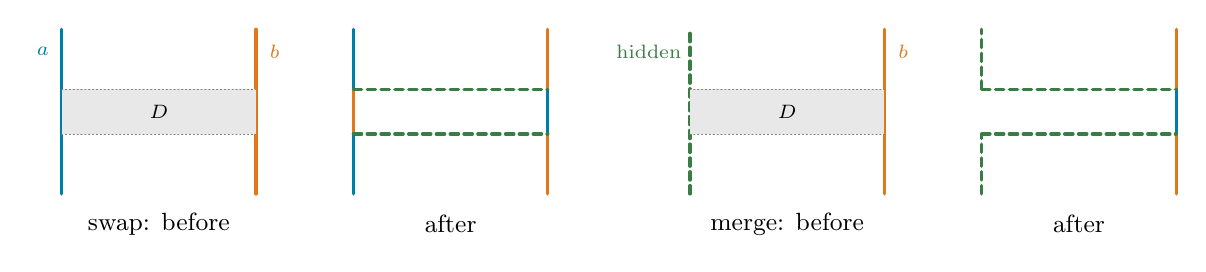
\begin{tikzpicture}[scale=.95,line cap=round,line join=round]
% swap, before
\begin{scope}
\draw[cutA,very thick] (0,0)--(0,2.2);
\draw[cutB,very thick] (2.6,0)--(2.6,2.2);
\fill[gray!18] (0,.8) rectangle (2.6,1.4);
\draw[gray,thin,densely dotted] (0,.8)--(2.6,.8) (0,1.4)--(2.6,1.4);
\node[font=\scriptsize] at (1.3,1.1) {$D$};
\node[font=\scriptsize,cutA] at (-.25,1.9) {$a$};
\node[font=\scriptsize,cutB] at (2.85,1.9) {$b$};
\node[font=\small] at (1.3,-.4) {swap: before};
\end{scope}
\begin{scope}[xshift=3.9cm]
\draw[cutA,very thick] (0,0)--(0,.8) (0,1.4)--(0,2.2) (2.6,.8)--(2.6,1.4);
\draw[cutB,very thick] (2.6,0)--(2.6,.8) (2.6,1.4)--(2.6,2.2) (0,.8)--(0,1.4);
\draw[hid,very thick,densely dashed] (0,.8)--(2.6,.8) (0,1.4)--(2.6,1.4);
\node[font=\small] at (1.3,-.4) {after};
\end{scope}
% merge, before
\begin{scope}[xshift=8.4cm]
\draw[hid,very thick,densely dashed] (0,0)--(0,2.2);
\draw[cutB,very thick] (2.6,0)--(2.6,2.2);
\fill[gray!18] (0,.8) rectangle (2.6,1.4);
\draw[gray,thin,densely dotted] (0,.8)--(2.6,.8) (0,1.4)--(2.6,1.4);
\node[font=\scriptsize] at (1.3,1.1) {$D$};
\node[font=\scriptsize,hid] at (-.55,1.9) {hidden};
\node[font=\scriptsize,cutB] at (2.85,1.9) {$b$};
\node[font=\small] at (1.3,-.4) {merge: before};
\end{scope}
\begin{scope}[xshift=12.3cm]
\draw[hid,very thick,densely dashed] (0,0)--(0,.8) (0,1.4)--(0,2.2);
\draw[cutB,very thick] (2.6,0)--(2.6,.8) (2.6,1.4)--(2.6,2.2);
\draw[cutA,very thick] (2.6,.8)--(2.6,1.4);
\draw[hid,very thick,densely dashed] (0,.8)--(2.6,.8) (0,1.4)--(2.6,1.4);
\node[font=\small] at (1.3,-.4) {after};
\end{scope}
\end{tikzpicture}
\caption{Flipping a band $D$ in a face. Blue: in $\A$ only; orange: in $\B$
only; dashed green: in both (hidden). \emph{Swap}: each family is pushed
across the band, and neither changes its shape. \emph{Merge}: $\A$ is
pushed across the band, while the two curves of $\B$ at its ends are cut
and joined to each other along the walls.}
\label{fig:moves}
\end{figure}

\begin{lemma}[The two moves]\label{lem:moves}
Let $D$ be a band from $e_1$ to $e_2$ in a configuration.
\begin{enumerate}[label=\textup{(\alph*)}]
\item \emph{Swap.} If $e_1$ is $a$-visible and $e_2$ is $b$-visible, the
  flip is a configuration in which each arc of $\A$ and each component of
  $\B$ is the old one up to an isotopy of $Q$ that moves no endpoint.
  Afterwards $e_1$ is $b$-visible and $e_2$ is $a$-visible.
\item \emph{Merge.} If $e_1$ is hidden and $e_2$ is $b$-visible, the flip
  is a configuration in which each arc of $\A$ is the old one up to such an
  isotopy, and $\B'$ arises from $\B$ by cutting it at $e_1$ and at $e_2$
  and joining the four ends along the two walls.
\end{enumerate}
\end{lemma}
\begin{proof}
In both cases $e_1\subset\A$ and $e_2\not\subset\A$, so $\A'$ is $\A$ with
the segment $e_1$ replaced by the path $w_1\cup e_2\cup w_2$, which has the
same ends and meets $\A$ nowhere else. This is a push of one arc across the
disc $D$, so (C1) holds. In (a), $e_2\subset\B$ and $e_1\not\subset\B$, and
$\B'$ is a push of $\B$ in the same way. In (b), both ends lie in $\B$, and
$\B'=(\B\setminus(e_1\cup e_2))\cup w_1\cup w_2$ up to closure, which is the
surgery described; it is again a compact $1$-manifold with the same
endpoints. (C3) holds since $\A'\triangle\B'=\A\triangle\B$. In a swap the new
common points are the two walls, which end at the ends of $e_1$ and $e_2$,
interior points of edges of $\Gamma$. In a merge $e_1$ leaves both
families, so the hidden cut through it falls into two parts, and each part
together with one wall is a new hidden cut, from an old switch to an end
of $e_2$. For (C4), a flip takes a subarc out of
$\A$ only in a swap, where $e_1$ is a proper part of an $a$-visible piece.
\end{proof}

Cutting two different components of a $1$-manifold and joining the ends the
other way has a simple effect. A closed curve and any other component
become one component. Two arcs become two arcs, each made of a half of
each old one.

\subsection{Joining two curves of the second sheet}

\begin{lemma}[Surgery]\label{lem:surgery}
Let $(\A,\B)$ be a configuration, and let $\beta_1\ne\beta_2$ be components
of $\B$ that can be joined by a path in $Q$ meeting $\B$ only in its two
ends. Then there is a configuration $(\A',\B')$ in which $\B'$ arises from
$\B$, up to an isotopy of $Q$ that moves no endpoint, by cutting $\beta_1$
and $\beta_2$ once each and joining each end of $\beta_1$ to an end of
$\beta_2$.
\end{lemma}
\begin{proof}
We use swaps to bring a $b$-visible piece of $\beta_1$ and a hidden piece of
$\beta_1$ or $\beta_2$ to the boundary of one face, next to a piece of the
other curve of the right kind, and then merge.

Two tools first. Let $h$ be a hidden cut on the boundary of a face $U$,
ending at a switch $p$ on an edge $f$, and let $f_a$, $f_b$ be the
$a$-visible and $b$-visible parts of $f$ at $p$ (Lemma~\ref{lem:local}a).
Near $p$ the face $U$ lies between $h$ and one of $f_a$, $f_b$. Inside a
small neighbourhood of $p$, on the side of $f$ away from $h$, flip a band
from a segment $e_1\subset f_a$ to a segment $e_2\subset f_b$. This is a
swap. Afterwards $e_1$ is $b$-visible and belongs to the component of $\B$
through $h$, to which it is joined by a wall and the stretch of $f_b$ up to
$p$; and $e_2$ is $a$-visible. Whichever of $f_a$, $f_b$ the face $U$
borders, it now borders a piece of the other kind as well. (If the far
side of $f$ is $U$ itself, the band only splits a small disc at $p$ off
$U$.) With Lemma~\ref{lem:local}(c) this gives, for any face $U$:
\begin{itemize}
\item[(T1)] if a component $\beta$ of $\B$ has a piece on $\bd U$, then
  after at most one swap it has a $b$-visible piece on $\bd U$;
\item[(T2)] after at most one swap, $\bd U$ contains an $a$-visible piece.
\end{itemize}

Now let $\rho$ be the given path. We may take it simple, crossing $G$
transversally, and staying away from switches, touchings and $\bd Q$; an
end that sits at such a point is slid a little along $\B$. The swaps of
(T1) and (T2) are made in neighbourhoods of switches that $\rho$ avoids.
Every flip below subdivides faces; by ``the face $U_i$'' we always mean the
face of the current graph that contains the corresponding stretch of
$\rho$. The new walls lie in thin bands around stretches of $\rho$
already used, so the rest of $\rho$ still meets $\B$ nowhere. Its interior misses $\B$, so it crosses
only $a$-visible pieces, say $x_1,\dots,x_m$ in this order, and it passes
through faces $U_0,\dots,U_m$. It starts on a piece $g$ of $\beta_1$ on
$\bd U_0$ and ends on a piece $d$ of $\beta_2$ on $\bd U_m$.

\emph{Walking.} By (T1) we may assume that $g$ is $b$-visible, moving the
start of $\rho$ inside $U_0$. Flip a thin band along $\rho$ in $U_0$, from $g$ to a short segment $s_1$ of $x_1$ around the point where $\rho$
crosses it: a swap, after which $s_1$ is a
$b$-visible piece of (the pushed) $\beta_1$, and it borders $U_1$. Repeat
in $U_1$ with a thinner band from the middle of $s_1$ to a segment
$s_2\subset x_2$, and so on. The bands are disjoint, since $\rho$ is
simple. After $m$ swaps a $b$-visible piece $e$ of $\beta_1$ lies on
$\bd U_m$, and so does $d$.

\emph{Joining.} If $d$ is hidden, flip a band in $U_m$ from $d$ to $e$: a
merge, which cuts $\beta_2$ at $d$ and $\beta_1$ at $e$ and joins them.
If $d$ is $b$-visible, we first need an $a$-visible piece $y$ on
$\bd U_m$. If $m\ge1$ the part of $x_m$ beside $s_m$ is one; if $m=0$, (T2) gives one.
Flip a band $D'$ in $U_m$ from $y$ to part of $e$, a swap. Its walls are
now hidden pieces of $\beta_1$. The band cuts $U_m$ into at most two
faces, each bordering a wall, and $d$ lies on the boundary of one of them.
In that face, flip a band from the wall to $d$: a merge of $\beta_1$ and
$\beta_2$.

Every step but the last moved each component of $\B$ by an isotopy, and
the last is the surgery.
\end{proof}

\subsection{Cutting the first sheet}

\begin{lemma}\label{lem:start}
A configuration exists.
\end{lemma}
\begin{proof}
We draw $\A$ and then let $\B=\overline{\Gamma\triangle\A}$. For this to be
a $1$-manifold, $\A$ has to pass every touching, entering and leaving
along pieces of $\Gamma$; it must begin and end along $\Gamma$; and it must
never cross an edge of $\Gamma$ in a single point.

Choose the following \emph{stations}, pairwise disjoint and short: at each
touching, a path along two of the four pieces of $\Gamma$ that meet there;
on each edge of $\Gamma$, a segment in its interior; and at each $T_i$ and
$B_i$, an initial segment of the edge of $\Gamma$ ending there.

The first arc $a_1$ starts at $T_1$ with its station, visits every station
that is not at some $T_i$ or $B_i$ with $i\ge2$, running through each from
end to end, and ends with the station at $B_1$. Between stations it runs through $\intr Q$, avoiding the touchings and
the other stations. This is possible: the part of $a_1$ drawn so far is an
arc attached to $\bd Q$, the remaining stations are disjoint arcs, and the
complement of all of these in $\intr Q$ is connected, so the next station
can always be reached. Wherever such a connecting path would cross an edge
of $\Gamma$, we let it run along the edge for a short stretch before
leaving on the other side. The points $T_i$, $B_i$ with $i\ge2$ now lie on
one side of $a_1$, on the boundary of a disc, in an order that allows
disjoint arcs $a_i$ from $T_i$ to $B_i$ inside it. Draw these, each
beginning and ending with its station and crossing edges of $\Gamma$ only
in the same way, by a short stretch along the edge.

(C1) holds by construction and (C4) by the stations on the edges. Let
$\B=\overline{\Gamma\triangle\A}$. At a point of an edge of $\Gamma$ where
$\A$ arrives or leaves, $\B$ consists of the rest of the edge and the part
of $\A$ off $\Gamma$: two pieces. At a touching, $\B$ consists of the two
pieces of $\Gamma$ that $\A$ does not use. Elsewhere $\B$ is locally a
piece of $\Gamma$ or of $\A$. Near $T_i$ and $B_i$ it is empty, and near
$L_j$ and $R_j$ it is the edge of $\Gamma$ ending there. So $\B$ is a
compact $1$-manifold with the endpoints required in (C2), and (C3) holds
with the stretches of $\A$ off $\Gamma$ as hidden cuts.
\end{proof}

\subsection{Proof of sufficiency}

Start from the configuration of Lemma~\ref{lem:start}. In any
configuration $\B$ has exactly $l$ arcs, since it has $2l$ endpoints, and
some closed curves.

\emph{Closed curves.} Let $\gamma$ be a closed curve of $\B$. Since
$l\ge1$, $\B$ has another component. Take a path from $\gamma$ to
$\B\setminus\gamma$, and cut it down to the stretch between its last
point on $\gamma$ and the first point of $\B$ after that. This stretch
joins $\gamma$ to another component $\beta$ and meets $\B$ only in its
ends. By Lemma~\ref{lem:surgery} we may cut and join $\gamma$ and $\beta$,
which leaves one closed curve fewer. Repeat until $\B$ consists of $l$
arcs.

\emph{Pairing.} Suppose $\B$ consists of $l$ disjoint arcs, and that for
some $j\ge 1$ the arcs at $L_1,\dots,L_{j-1}$ end at
$R_1,\dots,R_{j-1}$ respectively. Let $\omega'$ be the arc at $L_j$ and
$\omega$ the arc at $R_j$. If they are the same arc, there is nothing to
do. Otherwise let $x$ and $y$ be their other ends. Consider the region of
$Q\setminus\B$ just below the arc from $L_{j-1}$ to $R_{j-1}$, or below $T$
if $j=1$. Its boundary runs down $L$ to $L_j$ and down $R$ to $R_j$, so
both $\omega'$ and $\omega$ lie on it, and a path through the region joins
them. Apply Lemma~\ref{lem:surgery}. The two new arcs each consist of half
of $\omega'$ and half of $\omega$, so they pair the four ends either as
$\{L_jR_j,\ xy\}$ or as $\{L_jy,\ R_jx\}$. Going around $\bd Q$, no end of
an arc of $\B$ other than those of the first $j-1$ arcs lies between $L_j$
and $R_j$ on the upper side. Since $\omega'$ and $\omega$ were disjoint, the
four ends therefore lie in the cyclic order $L_j,R_j,y,x$. In this order
the chords $L_jy$ and $R_jx$ cross, and disjoint arcs in a disc cannot
realize crossing chords. So the new arcs are $L_jR_j$ and $xy$: the arc at
$L_j$ now ends at $R_j$, and the first $j-1$ arcs were not touched.

By induction on $j$ we reach a configuration in which the arc at $L_j$
ends at $R_j$ for every $j$. Here we use $t_L=t_R$. By
Lemma~\ref{lem:done}, $M$ is weavable. \qed

\begin{remark}[Corners]
Designers also let two cuts end together in a corner of the square. If
ends of arcs are allowed at corners, with at most one arc of each family at
each, the criterion changes only there: at most two pieces of $\Gamma$ may
end at a corner, and the counts in (iii) are taken after deciding, in one
of at most two ways per corner, which families end there. This follows from
Theorem~\ref{thm:main} by moving every corner end a little way along a
side, weaving, and moving it back.
\end{remark}

\begin{remark}[Proof by picture]
The proof is a procedure one can watch. Cut the first sheet along any
curves that follow the picture's boundary for a stretch at every edge and
through every touching. What is left of the boundary, together with the
stretches where the first cut strayed, is what the second sheet must cut:
a few arcs and many loops. A sheet cannot be cut along a loop. Each loop
is then opened into a neighbouring curve by a narrow band whose two walls
are cut in both sheets, and so vanish from the picture.
\end{remark}

\section{How many hidden cuts?}

Hidden cuts cost the weaver: each is a place where two strips must be
threaded through each other exactly, and thin paper tears there. Let
$h^*(M)$ be the least number of hidden cuts in a weave with picture $M$.
The proof above uses a number of them that is polynomial in the size of
$\Gamma$ but far from least. Two counting arguments bound $h^*$ from below.

\begin{lemma}[Meetings]\label{lem:meet}
A weave whose picture has $t$ touchings has at least $kl-t$ hidden cuts.
\end{lemma}
\begin{proof}
An arc $a$ from $T$ to $B$ and an arc $b$ from $L$ to $R$ meet. If a
component of $a\cap b$ is a single point $p$, then near $p$ both arcs are
visible on both sides of $p$, so four pieces of $\Gamma$ meet at $p$ and it
is a touching. Every other component is a hidden cut. At most one arc of
each family passes through a point, so each touching and each hidden cut
serves one pair $(a,b)$, and there are $kl$ pairs.
\end{proof}

\begin{lemma}[Islands]\label{lem:island}
Let $S$ be a nonempty union of components of $\Gamma$ that do not meet
$\bd Q$. The number of hidden cuts with exactly one end on $S$ is even and
at least two.
\end{lemma}
\begin{proof}
Some arc $a$ of $\A$ has a visible piece on $S$: an arc of $\A$ passes
every touching, and a component without touchings is a closed curve, which
cannot lie entirely in arcs of $\B$, since an arc contains no closed
curve. The ends of $a$ are on $\bd Q$,
off $S$, and $a$ can pass between $S$ and the rest of $\Gamma$ only along
hidden cuts with one end on $S$. It does so an even, positive number of
times. Each hidden cut lies on one arc of $\A$; sum over these arcs.
\end{proof}

\paragraph{Grids.}
The bound of Lemma~\ref{lem:meet} is attained exactly by the pictures
obtained from a grid. Take $k$ vertical and $l$ horizontal lines. At each
of the $kl$ crossings either keep the crossing, or \emph{smooth} it in one
of the two ways, joining the four ends in pairs without crossing.

\begin{proposition}\label{prop:grid}
A picture with $t$ touchings has $h^*=kl-t$ if and only if its boundary is
obtained, up to a homeomorphism of $Q$ that maps each side to itself, from
the $k\times l$ grid by keeping $t$ crossings and smoothing the others.
\end{proposition}
\begin{proof}
Given such a smoothing, draw the lines and, at each smoothed crossing, let
the two lines run together along a short diagonal placed so that the
visible cuts form the chosen smoothing, as in Figure~\ref{fig:model}(a).
Conversely, with $kl-t$ hidden cuts the count in Lemma~\ref{lem:meet} is
exact: every arc of $\A$ meets every arc of $\B$ once, at a touching or
along a hidden cut. Shrinking each hidden cut to a point gives $k$ disjoint
arcs from $T$ to $B$ and $l$ from $L$ to $R$, any two meeting once, which
is a grid up to homeomorphism; and $\Gamma$ is the smoothing of it at the
points that were hidden cuts.
\end{proof}

\begin{corollary}[Combs]\label{cor:comb}
Let $C_m$ be a square in the middle of $Q$ with $m$ arms reaching each
side. Its boundary has $O(m)$ vertices and corners, $k=l=2m$ and no
touchings, so every weave of $C_m$ has at least $4m^2$ hidden cuts. The
number of hidden cuts needed is therefore not linear in the size of the
picture.
\end{corollary}

In fact $h^*(C_m)=4m^2$: a suitable smoothing of the $2m\times2m$ grid is
the comb \cite{note}. In the other direction, a more careful construction
than the one of Section~2 weaves every picture satisfying
Theorem~\ref{thm:main} with $O(n^2)$ hidden cuts, where $n$ is the size of
$\Gamma$ \cite{note}; by the combs this is the right order.

\section{No hidden cuts at all is hard}

\begin{theorem}\label{thm:hard}
It is NP-complete to decide whether a picture can be woven without hidden
cuts. Hence computing $h^*$ is NP-hard.
\end{theorem}

Without hidden cuts the two families simply share out the boundary:
$\A\cup\B=\Gamma$, each edge of $\Gamma$ lies in one of them, and both pass
through every touching. A proposed sharing is checked at once, so the
problem is in NP. For hardness we use Hamilton cycles in planar cubic
graphs, which are NP-complete to find \cite{gjt}.

\begin{lemma}\label{lem:edge}
It is NP-complete to decide whether a plane cubic graph has a Hamilton
cycle through a given edge.
\end{lemma}
\begin{proof}
Take the cube on the $3$-bit strings, delete the edge $000$--$100$, and
join $000$ and $100$ to the two vertices of degree $2$ of a diamond ($K_4$
less an edge). Call the result $Y$ and the new edge at $000$ $e'$. Every
Hamilton cycle of $Y$ must enter and leave the diamond, so it uses $e'$.
Let $X=Y-001$, with terminals $000$, $011$, $101$, the neighbours of
$001$. A Hamilton path of $X$ between two terminals closes through $001$ to
a Hamilton cycle of $Y$, so it uses $e'$; and each pair of terminals is
joined by such a path, as one checks by hand. Now replace a vertex $v$ of
a plane cubic graph $H$ by $X$, attaching the terminals to the neighbours
of $v$ in the right cyclic order. The result $H'$ is plane and cubic. A
Hamilton cycle of $H'$ crosses the three edges at $X$ exactly twice, so it
restricts to a Hamilton path of $X$ and contracts to a Hamilton cycle of
$H$; conversely every Hamilton cycle of $H$ expands. So $H'$ has a
Hamilton cycle through $e'$ if and only if $H$ is Hamiltonian.
\end{proof}

\begin{figure}[ht]
\centering
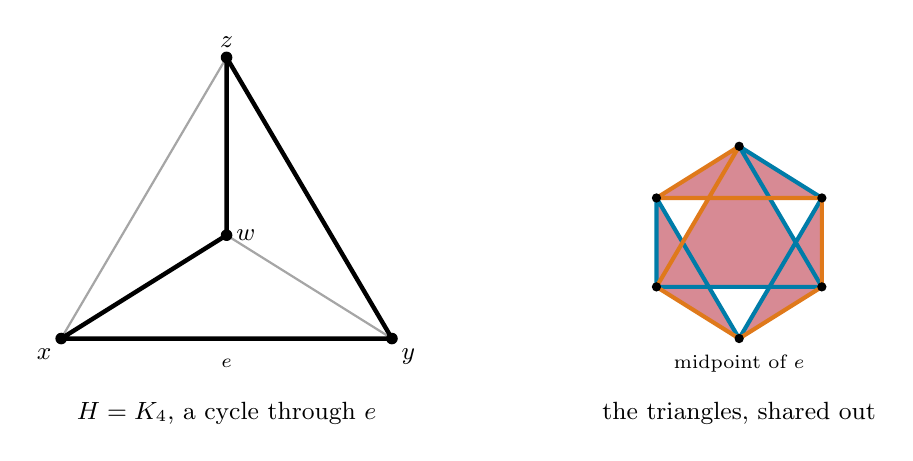
\begin{tikzpicture}[scale=1.05,line cap=round,line join=round]
\begin{scope}
\coordinate (x) at (0,0); \coordinate (y) at (4,0);
\coordinate (z) at (2,3.4); \coordinate (w) at (2,1.25);
\coordinate (xy) at (2,0); \coordinate (yz) at (3,1.7);
\coordinate (zx) at (1,1.7); \coordinate (wx) at (1,.625);
\coordinate (wy) at (3,.625); \coordinate (wz) at (2,2.325);
\draw[gray!70,thick] (x)--(y)--(z)--cycle (w)--(x) (w)--(y) (w)--(z);
\draw[black,line width=1.6pt] (x)--(y)--(z)--(w)--cycle;
\foreach \p/\n/\q in {x/x/below left,y/y/below right,z/z/above,w/w/right}
  {\fill (\p) circle (2pt); \node[font=\small,\q] at (\p) {$\n$};}
\node[font=\scriptsize] at (2,-.3) {$e$};
\node[font=\small] at (2,-.9) {$H=K_4$, a cycle through $e$};
\end{scope}
\begin{scope}[xshift=6.2cm]
\coordinate (x) at (0,0); \coordinate (y) at (4,0);
\coordinate (z) at (2,3.4); \coordinate (w) at (2,1.25);
\coordinate (xy) at (2,0); \coordinate (yz) at (3,1.7);
\coordinate (zx) at (1,1.7); \coordinate (wx) at (1,.625);
\coordinate (wy) at (3,.625); \coordinate (wz) at (2,2.325);
\fill[paper!55] (xy)--(zx)--(wx)--cycle;
\fill[paper!55] (xy)--(yz)--(wy)--cycle;
\fill[paper!55] (yz)--(zx)--(wz)--cycle;
\fill[paper!55] (wx)--(wy)--(wz)--cycle;
\draw[cutA,line width=1.5pt] (zx)--(xy)--(yz)--(wz)--(wy)--(wx)--cycle;
\draw[cutB,line width=1.5pt] (xy)--(wx)--(wz)--(zx)--(yz)--(wy)--cycle;
\foreach \p in {xy,yz,zx,wx,wy,wz} {\fill (\p) circle (1.6pt);}
\node[font=\scriptsize] at (2,-.3) {midpoint of $e$};
\node[font=\small] at (2,-.9) {the triangles, shared out};
\end{scope}
\end{tikzpicture}
\caption{The reduction for $H=K_4$. Each vertex becomes a triangle, and two
triangles touch at the middle of their common edge. Opened at the midpoint
of $e$ and stretched to the four sides of $Q$, this is a picture. Its
boundary can be shared between the two sheets, blue and orange, exactly
when $H$ has a Hamilton cycle through $e$: each sheet's cut follows the
cycle, and turns back where the cycle leaves out an edge.}
\label{fig:k4}
\end{figure}

\paragraph{The triangle picture.}
Let $H$ be a plane cubic graph and $e=xy$ an edge. For each vertex $z$ let
$\Delta_z$ be the triangle whose corners are the midpoints of the three
edges at $z$, drawn inside a neighbourhood of $z$ so that triangles of
adjacent vertices touch at the midpoint of their common edge and nowhere
else (Figure~\ref{fig:k4}). Now move the midpoint of $e$ to infinity: its
four pieces end at one point on each of $T$, $R$, $B$, $L$, and
$\Delta_x$, $\Delta_y$ become regions holding two opposite corners of
$Q$. The result is a picture $M(H,e)$ with $k=l=1$, of size linear in $H$,
in which every other midpoint is a touching.

\begin{lemma}\label{lem:claim}
$M(H,e)$ can be woven without hidden cuts if and only if $H$ has a
Hamilton cycle through $e$.
\end{lemma}
\begin{proof}
Without hidden cuts, the arc of $\A$ and the arc of $\B$ cover $\Gamma$,
each edge once, and each passes every touching once. Joined at infinity
they are two closed curves through all the midpoints, crossing at the
midpoint of $e$.

Suppose such a sharing exists. No triangle has all three sides in one
family, as they would close up. So each $\Delta_z$ has two sides in one
family, meeting at a corner where that family turns back off $\Delta_z$,
while the other family turns back off the triangle on the other side of
that corner. The edges of $H$ at whose midpoints this happens form a
perfect matching $N$. In each triangle both families run between the
midpoints of the two edges not in $N$, so each family follows
$C=E(H)\setminus N$ through every vertex. Each family is one closed curve,
so $C$ is a Hamilton cycle; and $e\in C$, because the families cross at its
midpoint instead of turning back.

Conversely let $C$ be a Hamilton cycle through $e$ and $N$ its complement.
For each edge $zw$ of $N$, give the two sides of $\Delta_z$ at its midpoint
to one family and the two sides of $\Delta_w$ there to the other; the third
side of each triangle goes to the family that did not get the other two.
Each family then follows $C$ through every triangle and passes every
midpoint once, so each is a single closed curve. Cut at infinity, they are
an arc from $T$ to $B$ and an arc from $L$ to $R$ that share out $\Gamma$.
\end{proof}

Lemmas~\ref{lem:edge} and~\ref{lem:claim} prove Theorem~\ref{thm:hard}.
Lemma~\ref{lem:claim} is a form of Kotzig's theorem that a cubic graph is
Hamiltonian exactly when its line graph splits into two Hamilton cycles.
The contrast with Theorem~\ref{thm:main} is the point: whether a picture
can be woven is easy, and whether it can be woven \emph{simply} is hard.

\section{The smallest pictures}

Although $h^*$ is hard in general, it can be computed for the pictures
people weave. A weave is determined, up to homeomorphism, by the order of
the switches along each edge of $\Gamma$, the family of each piece between
them, and the pairing of the switches by hidden cuts inside each
face, together with the side on which each hidden cut passes the holes of
its face. A
weave with $h$ hidden cuts has at most $2h$ switches, so a search over
these data with at most $2(h-1)$ switches per edge that finds nothing
proves that $h$ hidden cuts are needed. Such a search, with the two lemmas
of Section~3 as lower bounds, settles the pictures of
Table~\ref{tab:small} and almost all the designs on \url{https://juleflet.dk},
where the designers' own hearts turn out to use the fewest hidden cuts
possible \cite{note}.

\begin{table}[ht]
\centering
\begin{tabular}{@{}lccccl@{}}
\toprule
Picture & $k$ & $l$ & touchings & $h^*$ & no fewer, by\\
\midrule
Cross (two cuts crossing) & 1 & 1 & 1 & 0 & \\
$3\times3$ checkerboard & 2 & 2 & 4 & 0 & \\
Diagonal band & 1 & 1 & 0 & 1 & Lemma~\ref{lem:meet}\\
Island beside a cross & 1 & 1 & 1 & 2 & Lemma~\ref{lem:island}\\
Plus sign & 2 & 2 & 0 & 4 & Lemma~\ref{lem:meet}\\
Necklace with a pearl & 1 & 1 & 4 & 4 & Lemma~\ref{lem:island}, twice\\
Four islands & 1 & 1 & 1 & 5 & Lemma~\ref{lem:island}, for every set of islands\\
Rings inside rings (three) & 1 & 1 & 8 & 6 & Lemma~\ref{lem:island}, three times\\
\bottomrule
\end{tabular}
\caption{The least number of hidden cuts for some small pictures
\cite{note}. A boundary that fails to cross where the grid would cross
costs one hidden cut for each crossing left out; a single island costs
two, and several islands can share.}
\label{tab:small}
\end{table}

For $k=l=1$ the table can be read as the start of a list. With no hidden
cut the two cuts cross or touch at every meeting, and the pictures are the
cross and its relatives in which the two curves touch several times. With
one hidden cut and no touching, Proposition~\ref{prop:grid} gives exactly
the two diagonal bands. With two hidden cuts the first island appears. Four
islands need only five, not eight: one pair of hidden cuts can string
several islands together.

\paragraph{Open questions.}
Is $h^*=kl-t$ decidable in polynomial time? Proposition~\ref{prop:grid}
turns it into a question about smoothings of a grid, which a transfer
matrix answers in time exponential only in $\min(k,l)$. And how well can
$h^*$ be approximated?

\begin{thebibliography}{9}
\bibitem{mogensen}
T.~Mogensen, \emph{Braided Christmas Hearts}, 2021.
\url{https://hjemmesider.diku.dk/~torbenm/hearts.pdf}
\bibitem{gjt}
M.~R.~Garey, D.~S.~Johnson and R.~E.~Tarjan, The planar Hamiltonian circuit
problem is NP-complete, \emph{SIAM J.\ Comput.}\ 5 (1976), 704--714.
\bibitem{note}
T.~D.~Ahle, \emph{Alternating-weave representability: a local criterion},
working note with computations, October 2026.
\end{thebibliography}
\end{document}
